\begin{Pro}
    A partir de las siguientes instrucciones:
\begin{verbatim}
y = 1;
x = 10 + (y - 1);
while (x < y) {
    y += 1;
}
\end{verbatim}
\begin{enumerate}
    \item[(a)] Traduce el programa a código de tres direcciones.
    \item[(b)] Usa el formato de cuádruples para guardar las instrucciones.
    \item[(c)] Usa el formato de triples indirectos para guardar las instrucciones.
    \item[(d)] Define la función de ambiente $\Gamma$.
    \item[(e)] Utiliza las reglas de inferencia para checar que el programa está correctamente tipado.
    \item[(f)] Obtén sus conjuntos $succ$, $gen$, $kill$, $out$ e $in$.
    \item[(g)] Dibuja la gráfica de interferencia y asigna $n=3$ direcciones con el algoritmo de coloreado.
\end{enumerate}
\end{Pro}



\section*{Traducción de Código Intermedio}

\textbf{Código Fuente:}
\begin{verbatim}
y = 1;
x = 10 + (y - 1);
while (x < y) {
    y += 1;
}
\end{verbatim}

\subsection*{(a) Código de Tres Direcciones (TAC)}

Descomponemos las expresiones complejas en temporales ($t_n$) y utilizamos etiquetas ($L_n$) para el control de flujo del ciclo \texttt{while}.

\begin{center}
\begin{tabular}{r l l}
    \toprule
    \textbf{Línea} & \textbf{Instrucción} & \textbf{Comentario} \\
    \midrule
    (1) & $y = 1$ & Asignación inicial \\
    (2) & $t_1 = y - 1$ & Subexpresión paréntesis \\
    (3) & $t_2 = 10 + t_1$ & Suma con literal \\
    (4) & $x = t_2$ & Asignación a $x$ \\
    \midrule
    (5) & \textbf{L1:} & \textit{Inicio del ciclo (evaluación)} \\
    (6) & $t_3 = x < y$ & Evaluar condición \\
    (7) & \texttt{ifFalse} $t_3$ \texttt{goto} \textbf{L2} & Salida si condición falsa \\
    \midrule
    (8) & $t_4 = y + 1$ & Cuerpo: cálculo de incremento \\
    (9) & $y = t_4$ & Cuerpo: asignación \\
    (10) & \texttt{goto} \textbf{L1} & Regreso al inicio \\
    \midrule
    (11) & \textbf{L2:} & \textit{Fin del ciclo} \\
    \bottomrule
\end{tabular}
\end{center}

\subsection*{(b) Cuádruples}

Aquí representamos las etiquetas como instrucciones \texttt{LABEL} para mayor claridad, y usamos temporales explícitos.

\begin{center}
\begin{tabular}{|c|c|c|c|c|}
    \hline
    \textbf{Ref} & \textbf{Op} & \textbf{Arg1} & \textbf{Arg2} & \textbf{Resultado} \\
    \hline
    (0) & $=$ & $1$ & - & $y$ \\
    \hline
    (1) & $-$ & $y$ & $1$ & $t_1$ \\
    \hline
    (2) & $+$ & $10$ & $t_1$ & $t_2$ \\
    \hline
    (3) & $=$ & $t_2$ & - & $x$ \\
    \hline
    (4) & \texttt{LABEL} & - & - & \textbf{L1} \\
    \hline
    (5) & $<$ & $x$ & $y$ & $t_3$ \\
    \hline
    (6) & \texttt{ifFalse} & $t_3$ & - & \textbf{L2} \\
    \hline
    (7) & $+$ & $y$ & $1$ & $t_4$ \\
    \hline
    (8) & $=$ & $t_4$ & - & $y$ \\
    \hline
    (9) & \texttt{goto} & - & - & \textbf{L1} \\
    \hline
    (10) & \texttt{LABEL} & - & - & \textbf{L2} \\
    \hline
\end{tabular}
\end{center}

\subsection*{(c) Triples Indirectos}

Utilizamos dos estructuras. Los saltos en la tabla de triples hacen referencia a los índices definidos en la \textbf{Tabla de Instrucciones}.

\textbf{1. Tabla de Instrucciones (Apuntadores)}
\begin{center}
\begin{tabular}{|c|c|l|}
    \hline
    \textbf{Pos} & \textbf{Apunta a Triple} & \textbf{Nota} \\
    \hline
    $[0]$ & (0) & \\
    \hline
    $[1]$ & (1) & \\
    \hline
    $[2]$ & (2) & \\
    \hline
    $[3]$ & (3) & \\
    \hline
    $[4]$ & (4) & $\leftarrow$ Inicio \textbf{L1} \\
    \hline
    $[5]$ & (5) & \\
    \hline
    $[6]$ & (6) & \\
    \hline
    $[7]$ & (7) & \\
    \hline
    $[8]$ & (8) & \\
    \hline
\end{tabular}
\end{center}
\textit{Nota: La posición imaginaria $[9]$ representaría la salida del bucle (\textbf{L2}).}

\textbf{2. Tabla de Triples}
\begin{center}
\begin{tabular}{|c|c|c|c|}
    \hline
    \textbf{ID} & \textbf{Op} & \textbf{Arg1} & \textbf{Arg2} \\
    \hline
    (0) & \texttt{assign} & $y$ & $1$ \\
    \hline
    (1) & $-$ & $y$ & $1$ \\
    \hline
    (2) & $+$ & $10$ & (1) \\
    \hline
    (3) & \texttt{assign} & $x$ & (2) \\
    \hline
    (4) & $<$ & $x$ & $y$ \\
    \hline
    (5) & \texttt{ifFalse} & (4) & $[9]$ \\
    \hline
    (6) & $+$ & $y$ & $1$ \\
    \hline
    (7) & \texttt{assign} & $y$ & (6) \\
    \hline
    (8) & \texttt{goto} & $[4]$ & - \\
    \hline
\end{tabular}
\end{center}
\footnotesize{\textit{Explicación de saltos: El triple (5) salta a la posición [9] (salida) si la condición (4) es falsa. El triple (8) salta incondicionalmente a la posición [4], donde se re-evalúa la condición.}}


\section*{Checado de Tipos }

    \textbf{Definición del Ambiente $\Gamma$}

    Dado que las variables reciben valores enteros y operan aritméticamente, definimos el contexto como:
    \[
    \Gamma = \{ x : \texttt{int}, \quad y : \texttt{int} \}
    \]

    \textbf{Reglas de Inferencia y Verificación}

    Utilizaremos las siguientes reglas estándar:
    \begin{center}
    \small
    \textbf{(Op)} $\frac{\Gamma \vdash e_1 : \texttt{int} \quad \Gamma \vdash e_2 : \texttt{int}}{\Gamma \vdash e_1 \odot e_2 : \texttt{int}}$ \quad
    \textbf{(Rel)} $\frac{\Gamma \vdash e_1 : \texttt{int} \quad \Gamma \vdash e_2 : \texttt{int}}{\Gamma \vdash e_1 < e_2 : \texttt{bool}}$ \quad
    \textbf{(Assign)} $\frac{\Gamma(id) = \tau \quad \Gamma \vdash E : \tau}{\Gamma \vdash id = E : \texttt{ok}}$
    \end{center}

    Dividimos la demostración en 3 partes correspondientes a las sentencias del programa.

    \textbf{Parte 1: Primera Asignación ($y = 1$)}
    \[
    D_1: \frac{\Gamma(y) = \texttt{int} \quad \Gamma \vdash 1 : \texttt{int}}{\Gamma \vdash y = 1 : \texttt{ok}}
    \]

    \textbf{Parte 2: Segunda Asignación ($x = 10 + (y - 1)$)}
    Construimos el tipo de la expresión aritmética derecha:
    \[
    D_{expr}: \frac{\Gamma \vdash 10:\texttt{int} \quad \frac{\Gamma(y)=\texttt{int} \quad \Gamma \vdash 1:\texttt{int}}{\Gamma \vdash y-1 : \texttt{int}}}{\Gamma \vdash 10 + (y - 1) : \texttt{int}}
    \]
    
    Luego aplicamos la regla de asignación:
    \[
    D_2: \frac{\Gamma(x) = \texttt{int} \quad D_{expr}}{\Gamma \vdash x = 10 + (y - 1) : \texttt{ok}}
    \]

    \textbf{Parte 3: Ciclo While ($\texttt{while } (x < y) \{ y += 1 \}$)}
    
    Analizamos primero la condición ($C$):
    \[
    D_{cond}: \frac{\Gamma(x)=\texttt{int} \quad \Gamma(y)=\texttt{int}}{\Gamma \vdash x < y : \texttt{bool}}
    \]

    Analizamos el cuerpo ($S_{body}$), tratando $y += 1$ como $y = y + 1$:
    \[
    D_{body}: \frac{\Gamma(y)=\texttt{int} \quad \frac{\Gamma(y)=\texttt{int} \quad \Gamma \vdash 1:\texttt{int}}{\Gamma \vdash y+1 : \texttt{int}}}{\Gamma \vdash y = y + 1 : \texttt{ok}}
    \]

    Unimos ambos en la regla del While:
    \[
    D_3: \frac{D_{cond} \quad D_{body}}{\Gamma \vdash \texttt{while } (x < y) \{ \dots \} : \texttt{ok}}
    \]

    \textbf{Conclusión Final (Secuencia)}
    Unimos las tres sentencias ($D_1, D_2, D_3$) mediante la regla de secuencia (\textbf{Seq}):
    
    \[
    \frac{D_1 \quad D_2 \quad D_3}{\Gamma \vdash \text{Programa} : \texttt{ok}}
    \]
    
    $\therefore$ El programa está correctamente tipado bajo el ambiente $\Gamma$.





 \textbf{Conjuntos succ, gen, kill, in, out}

Realizamos el análisis de flujo de datos hacia atrás (bottom-up), comenzando desde el final del programa para propagar la vida de las variables.

\begin{center}
\renewcommand{\arraystretch}{1.4}
\setlength{\tabcolsep}{4pt}
\begin{tabular}{|c|l|c|c|c|c|c|}
    \hline
    \textbf{\#} & \textbf{Instrucción} & \textbf{succ} & \textbf{gen} & \textbf{kill} & \textbf{out} & \textbf{in} \\
    \hline
    11 & \texttt{L2:} & $\emptyset$ & $\emptyset$ & $\emptyset$ & $\emptyset$ & $\emptyset$ \\
    \hline
    10 & \texttt{goto L1} & $\{6\}$ & $\emptyset$ & $\emptyset$ & $\{x, y\}$ & $\{x, y\}$ \\
    \hline
    9 & \texttt{y = t4} & $\{10\}$ & $\{t_4\}$ & $\{y\}$ & $\{x, y\}$ & $\{t_4, x\}$ \\
    \hline
    8 & \texttt{t4 = y + 1} & $\{9\}$ & $\{y\}$ & $\{t_4\}$ & $\{t_4, x\}$ & $\{x, y\}$ \\
    \hline
    7 & \texttt{ifFalse t3...} & $\{8, 11\}$ & $\{t_3\}$ & $\emptyset$ & $\{x, y\}$ & $\{t_3, x, y\}$ \\
    \hline
    6 & \texttt{t3 = x < y} & $\{7\}$ & $\{x, y\}$ & $\{t_3\}$ & $\{t_3, x, y\}$ & $\{x, y\}$ \\
    \hline
    5 & \texttt{L1:} & $\{6\}$ & $\emptyset$ & $\emptyset$ & $\{x, y\}$ & $\{x, y\}$ \\
    \hline
    4 & \texttt{x = t2} & $\{5\}$ & $\{t_2\}$ & $\{x\}$ & $\{x, y\}$ & $\{t_2, y\}$ \\
    \hline
    3 & \texttt{t2 = 10 + t1} & $\{4\}$ & $\{t_1\}$ & $\{t_2\}$ & $\{t_2, y\}$ & $\{t_1, y\}$ \\
    \hline
    2 & \texttt{t1 = y - 1} & $\{3\}$ & $\{y\}$ & $\{t_1\}$ & $\{t_1, y\}$ & $\{y\}$ \\
    \hline
    1 & \texttt{y = 1} & $\{2\}$ & $\emptyset$ & $\{y\}$ & $\{y\}$ & $\emptyset$ \\
    \hline
\end{tabular}
\end{center}

\begin{itemize}
    \item \textbf{Línea 9 ($y = t_4$):} Aunque se reescribe $y$, la variable $x$ debe mantenerse viva en el conjunto $in$ porque se necesitará más adelante en el ciclo (línea 6), y la instrucción 9 no mata a $x$. Por eso $in[9] = \{t_4, x\}$.
    \item \textbf{Línea 7 (Salto condicional):} Tiene dos caminos posibles (entrar al cuerpo o salir). Su conjunto $out$ es la unión de la entrada del cuerpo ($in[8]=\{x,y\}$) y la salida del programa ($in[11]=\emptyset$).
    \item \textbf{Línea 1 ($y=1$):} Al inicio ($in[1]$), el conjunto es vacío, lo cual es correcto porque ninguna variable tiene un valor útil antes de empezar el programa.
\end{itemize}


\textbf{Gráfica de Interferencia y Asignación de Registros}

Basándonos en los conjuntos \textit{in} del inciso anterior, construimos la gráfica de interferencia. Dos nodos están conectados si las variables están vivas simultáneamente.

\textbf{Análisis de Grados:}
\begin{itemize}
    \item $deg(y) = 4$ (Vecinos: $x, t_1, t_2, t_3$)
    \item $deg(x) = 3$ (Vecinos: $y, t_3, t_4$)
    \item $deg(t_3) = 2$ (Vecinos: $x, y$)
    \item $deg(t_1), deg(t_2), deg(t_4) = 1$
\end{itemize}

\begin{center}
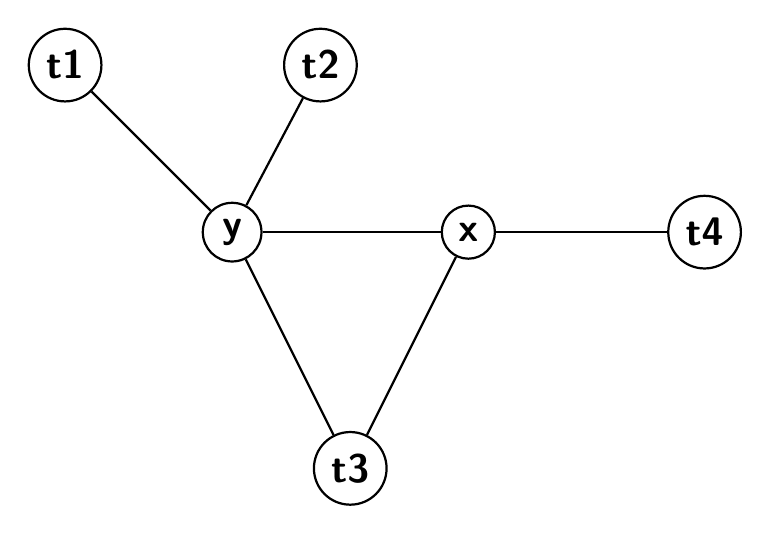
\begin{tikzpicture}[auto, node distance=3cm, thick, main/.style={circle, draw, font=\sffamily\Large\bfseries}]
  % Nodos
  \node[main] (y) {y};
  \node[main] (x) [right of=y] {x};
  \node[main] (t3) [below of=y, xshift=1.5cm] {t3};
  \node[main] (t1) [above left of=y] {t1};
  \node[main] (t2) [above right of=y, xshift=-1cm] {t2};
  \node[main] (t4) [right of=x] {t4};

  % Aristas (Interferencias)
  \draw (y) -- (x);
  \draw (y) -- (t3);
  \draw (x) -- (t3);
  
  \draw (y) -- (t1);
  \draw (y) -- (t2);
  
  \draw (x) -- (t4);
\end{tikzpicture}
\end{center}

\textbf{Asignación de Registros ($N=3$):}
Utilizando el algoritmo de coloreado por pila, obtenemos la siguiente distribución óptima:

\begin{center}
\renewcommand{\arraystretch}{1.3}
\begin{tabular}{|c|c|l|}
    \hline
    \textbf{Variable} & \textbf{Registro Asignado} & \textbf{Justificación} \\
    \hline
    $y$ & \textbf{R1} & Primer nodo coloreado. \\
    \hline
    $x$ & \textbf{R2} & Interfiere con $y$ (R1). \\
    \hline
    $t_3$ & \textbf{R3} & Interfiere con $y$ (R1) y $x$ (R2). \\
    \hline
    $t_4$ & \textbf{R1} & Interfiere solo con $x$ (R2). R1 está libre. \\
    \hline
    $t_2$ & \textbf{R2} & Interfiere solo con $y$ (R1). R2 está libre. \\
    \hline
    $t_1$ & \textbf{R2} & Interfiere solo con $y$ (R1). R2 está libre. \\
    \hline
\end{tabular}
\end{center}

El programa puede ejecutarse exitosamente con solo 3 registros físicos, reutilizando registros para las variables temporales no coincidentes.